\documentclass[paper=a4, fontsize=11pt]{scrartcl} % A4 paper and 11pt font size

%----------------------------------------------------------------------------------------
%	PACKAGES
%----------------------------------------------------------------------------------------
\usepackage[T1]{fontenc} % Use 8-bit encoding that has 256 glyphs
\usepackage{fourier} % Use the Adobe Utopia font for the document - comment this line to return to the LaTeX default
\usepackage[english]{babel} % English language/hyphenation
\usepackage{amsmath,amsfonts,amsthm} % Math packages
\usepackage{sectsty} % Allows customizing section commands
\usepackage{fancyhdr} % Custom headers and footers
\usepackage{tabularx, outlines, framed, varwidth, enumitem, graphicx, listings, color, qtree, float, subcaption, newfloat}
\usepackage[left=0.5in, right=0.5in, top=3in, bottom=.25in]{geometry}
\geometry{}

%----------------------------------------------------------------------------------------
%	SET CUSTOMIZATIONS AND FUNCTIONS
%----------------------------------------------------------------------------------------
\sectionfont{\centering \normalfont\scshape} % Make all sections centered, the default font and small caps
\pagestyle{fancyplain} % Makes all pages in the document conform to the custom headers and footers
\fancyhead{} % No page header - if you want one, create it in the same way as the footers below
\fancyfoot[L]{} % Empty left footer
\fancyfoot[C]{} % Empty center footer
\fancyfoot[R]{\thepage} % Page numbering for right footer
\renewcommand{\headrulewidth}{0pt} % Remove header underlines
\renewcommand{\footrulewidth}{0pt} % Remove footer underlines
\setlength{\headheight}{0pt} % Customize the height of the header

\DeclareFloatingEnvironment[fileext=lod]{diagram}

\numberwithin{equation}{section} % Number equations within sections (i.e. 1.1, 1.2, 2.1, 2.2 instead of 1, 2, 3, 4)
\numberwithin{figure}{section} % Number figures within sections (i.e. 1.1, 1.2, 2.1, 2.2 instead of 1, 2, 3, 4)
\numberwithin{table}{section} % Number tables within sections (i.e. 1.1, 1.2, 2.1, 2.2 instead of 1, 2, 3, 4)

\graphicspath{{./figures/}}
%\setlength\parindent{0pt} % Removes all indentation from paragraphs - comment this line for an assignment with lots of text

\makeatletter
	\newcommand*\variableheghtrulefill[1][.4\p@]
	{%
		\leavevmode
		\leaders \hrule \@height #1\relax \hfill
		\null
	}
\makeatother

\lstset
{
	language=C++,
%	basicstyle=\ttfamily,
%	keywordstyle=\color{blue}\ttfamily,
%	stringstyle=\color{red}\ttfamily,
%	commentstyle=\color{green}\ttfamily,
%	morecomment=[l][\color{magenta}]{\#}
	keywordstyle=\color{blue},
	stringstyle=\color{red},
	commentstyle=\color{green},
	morecomment=[l][\color{magenta}]{\#}
}

%----------------------------------------------------------------------------------------
%	USEFUL COMMANDS
%----------------------------------------------------------------------------------------
%	\makebox[\textwidth][c]{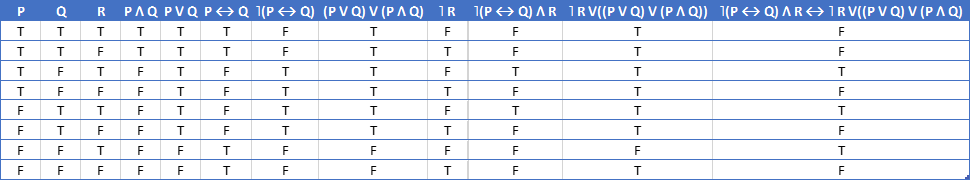
\includegraphics[width=.9\pagewidth]{p2-table}}

%	\newgeometry{top=.75in, bottom=.75in, left=.25in,right=.25in}
%	\newgeometry{top=.75in, bottom=.75in, left=1.25in,right=1.25in}

%	\lstinputlisting[firstline=4]{CMPSC360_Homework.cpp}

%\Tree
%	[.<root> [.<left> ][.<middle> ][.<right> ]]

%----------------------------------------------------------------------------------------
%	TITLE SECTION
%----------------------------------------------------------------------------------------

\newcommand{\horrule}[1]{\rule{\linewidth}{#1}} % Create horizontal rule command with 1 argument of height
% \title{Template: Homework 1}
\title{	
\normalfont \normalsize 
%\textsc{Rutgers University, Real Analysis I} \\ [25pt] % Your university, school and/or department name(s)
\horrule{0.5pt} \\[0.4cm] % Thin top horizontal rule
\huge STAT 463: Homework 7 \\ % The assignment title
\horrule{2pt} \\[0.5cm] % Thick bottom horizontal rule
}

\author{\textbf{\underline{Name:}}Kyle Salitrik | \textit{\textbf{\underline{ID\#:}} 997543474} | \textit{\textbf{\underline{PSU ID:}} kps168}} % Your name

\date{\normalsize\today} % Today's date or a custom date

\begin{document}

\maketitle % Print the title
\newgeometry{top=.75in, bottom=.75in, left=1.25in,right=1.25in}

%----------------------------------------------------------------------------------------
%	PROBLEM 1
%----------------------------------------------------------------------------------------



\section*{\variableheghtrulefill[.25ex]\quad Problem 1 \quad\variableheghtrulefill[.25ex]}
\subsection*{a)}
\makebox[\textwidth][c]{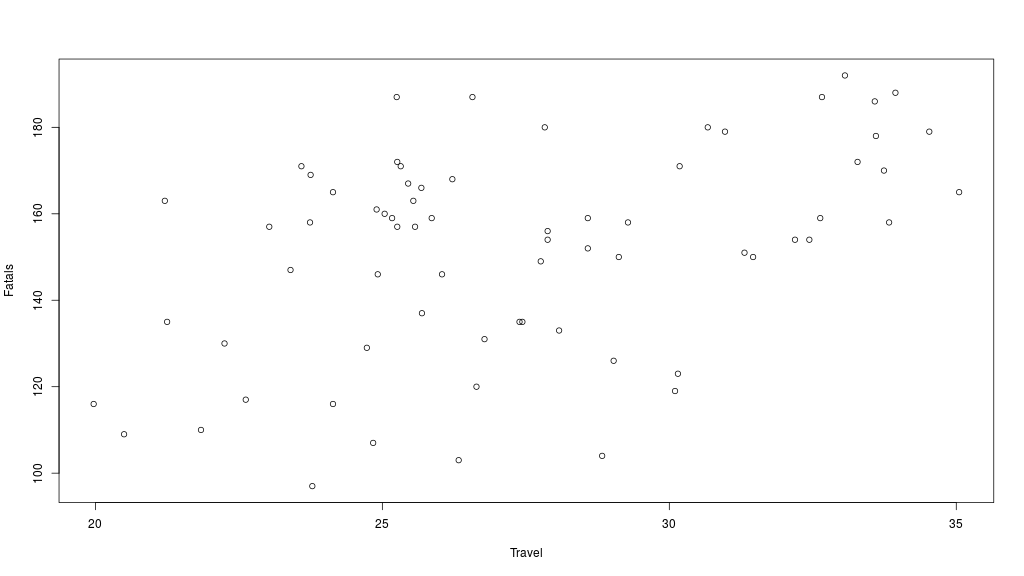
\includegraphics[scale=.5]{fatals_scatter.png}}

Performing a simple linear regression on the above data, the following information was obtained:
\begin{itemize}
	\item Intercept: 16.75850
	\item Intercept SE: 2.69288
	\item Slope: 0.07027
	\item Slope SE: 0.01754
\end{itemize}


\subsection*{b)}

Based on the ACF plots of the residuals, it appears that an ARIMA model of (1,0,0) would be a good fit.

\makebox[\textwidth][c]{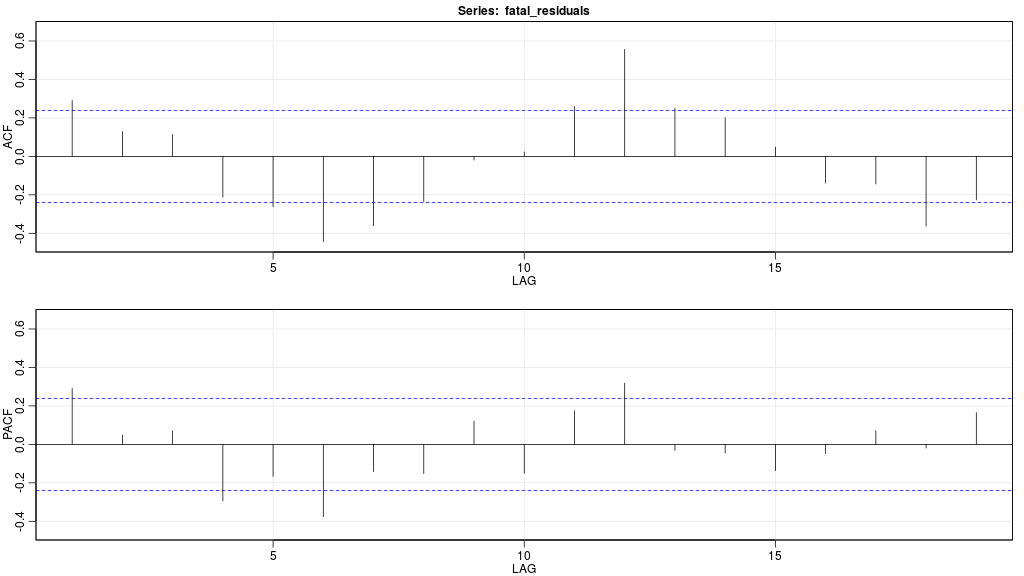
\includegraphics[scale=.5]{fatal_lm_residual_acf.png}}


\subsection*{c)}
Based on the arima model chosen, the diagnostic plots look okay. The Ljung-Box plot is fairly bad, but the QQ plot and ACF plots look alright.

\makebox[\textwidth][c]{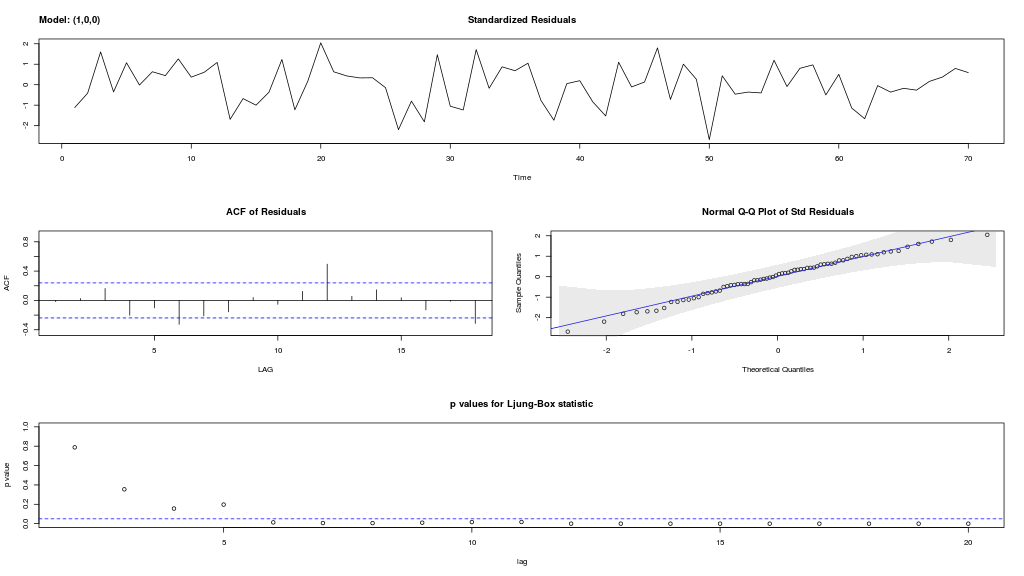
\includegraphics[scale=.5]{arima_residual_fit.png}}


\subsection*{d)}
After performing the adjustment regression, the following new slope and intercept information was obtained:

\begin{itemize}
	\item Intercept: 54.4500
	\item Intercept SE: 13.2512
	\item Slope: 2.7183
	\item Slope SE: 0.6784
\end{itemize}


\subsection*{e)}
Using the Cochrane-Orcutt function yielded the following results

\begin{itemize}
	\item Intercept: 86.08247
	\item Intercept SE: 23.98510
	\item Slope: 2.41695
	\item Slope SE: 0.85958
\end{itemize}



%----------------------------------------------------------------------------------------
%	PROBLEM 2
%----------------------------------------------------------------------------------------

\section*{\variableheghtrulefill[.25ex]\quad Problem 2 \quad\variableheghtrulefill[.25ex]}

The following R code was created for problem 2:

\lstinputlisting[language=]{listings/problem_2.txt}

%----------------------------------------------------------------------------------------
%	PROBLEM 2
%----------------------------------------------------------------------------------------

\section*{\variableheghtrulefill[.25ex]\quad Problem 3 \quad\variableheghtrulefill[.25ex]}

The forecasting yielded significantly different results for the two methods. The Cochrane-Orcutt model forecast was 55.29775 and the difference method forecast was 130.3482.

The residual for the CO method was -133.6638 and 234.8415 was the difference method's residual value.


\end{document}